\addcontentsline{toc}{chapter}{Jacob}

% Safely inserts your illustration full-bleed on its own page.
% This completely bypasses the page builder, headers, and geometry bugs!
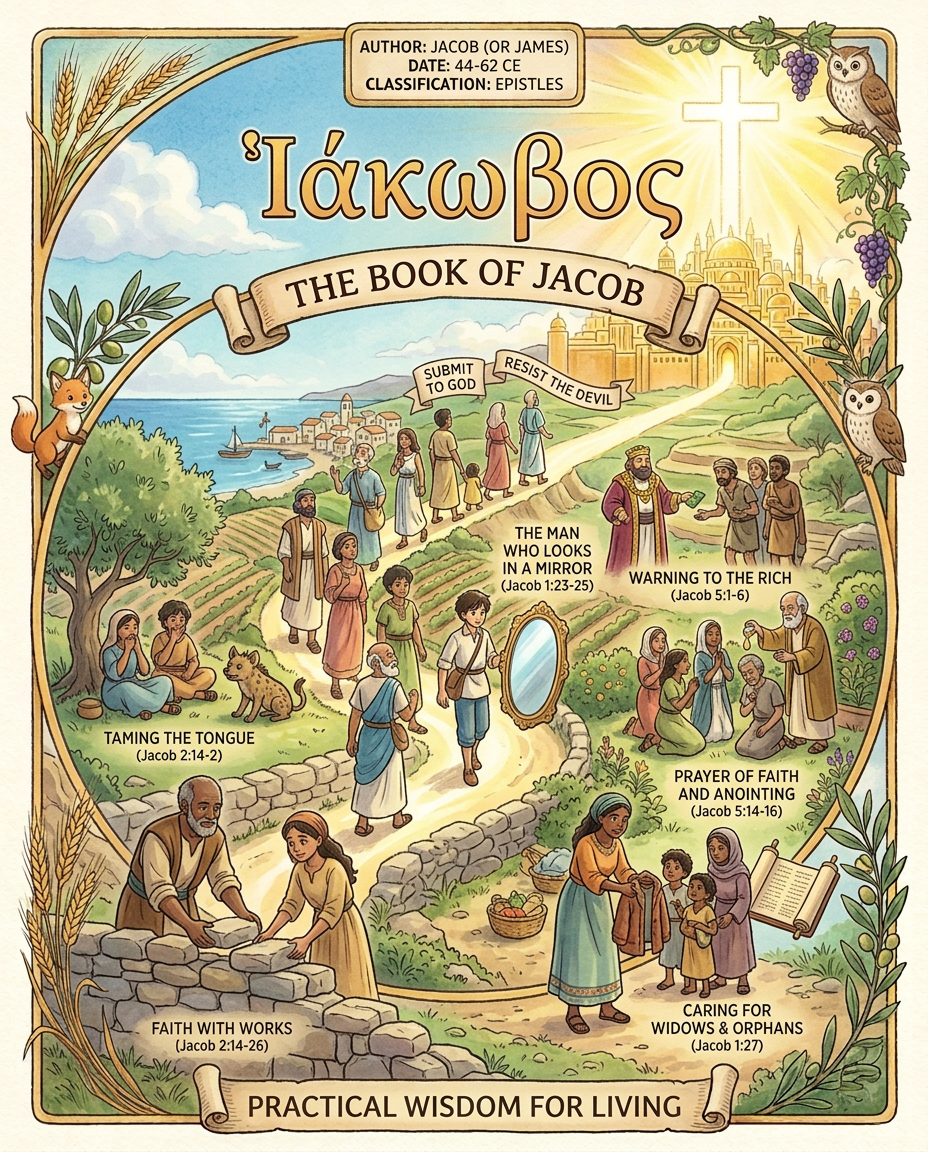
\includepdf[pages=1, fitpaper=false, width=\paperwidth, height=\paperheight, , keepaspectratio=false]{images/divider2/james2.png}
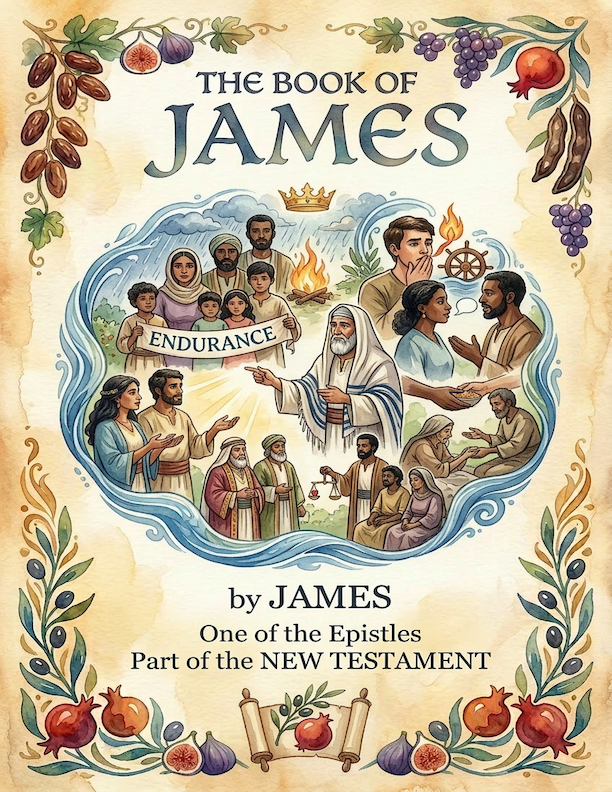
\includepdf[pages=1, fitpaper=false, width=\paperwidth, height=\paperheight, , keepaspectratio=false]{images/divider1/james.png}

\includepdf[pages=1, fitpaper=false, width=\paperwidth, height=\paperheight, , keepaspectratio=false]{images/8.5x11-Dot-Grid.png}

\includepdf[pages=1, fitpaper=false, width=\paperwidth, height=\paperheight, , keepaspectratio=false]{images/8.5x11-Dot-Grid.png}
\mybook{Jacob}
\vspace{-1.36in}


\mychapter{} \myverse*{}Jacob, a servant of God and of the Lord Yeshua the Messiah,\footnote{1:1 “Messiah” means “Anointed One”.} to the twelve tribes which are in the Diaspora: Greetings.

\myverse{}Count it all joy, my brothers,\footnote{1:2 The word for “brothers” here and where context allows may also be correctly translated “brothers
	and sisters” or “siblings.”} when you fall into various temptations,
\myverse{}knowing that the testing of your faith produces endurance.
\myverse{}Let endurance have its perfect work, that you may be perfect and complete, lacking
in nothing.

\myverse{}But if any of you lacks wisdom, let him ask of God, who gives to
all liberally and without reproach, and it will be given to him.
\myverse{}But let him ask in faith, without any doubting, for he who doubts is like a
wave of the sea, driven by the wind and tossed.
\myverse{}For that man shouldn’t think that he will receive anything from the Lord.
\myverse{}He is a double-minded man, unstable in all his ways.

\myverse{}Let the brother in humble circumstances glory in his high position;
\myverse{}and the rich, in that he is made humble, because like the flower in the grass,
he will pass away.
\myverse{}For the sun arises with the scorching wind and withers the grass; and the
flower in it falls, and the beauty of its appearance perishes. So the rich man will also fade away in
his pursuits.

\myverse{}Blessed is a person who endures temptation, for when he has been
approved, he will receive the crown of life which the Lord promised to those who love him.

\myverse{}Let no man say when he is tempted, “I am tempted by God,” for
God can’t be tempted by evil, and he himself tempts no one.
\myverse{}But each one is tempted when he is drawn away by his own lust and enticed.
\myverse{}Then the lust, when it has conceived, bears sin. The sin, when it is full
grown, produces death.
\myverse{}Don’t be deceived, my beloved brothers.
\myverse{}Every good gift and every perfect gift is from above, coming down from the
Father of lights, with whom can be no variation nor turning shadow.
\myverse{}Of his own will he gave birth to us by the word of truth, that we should be
a kind of first fruits of his creatures.

\myverse{}So, then, my beloved brothers, let every man be swift to hear,
slow to speak, and slow to anger;
\myverse{}for the anger of man doesn’t produce the righteousness of God.
\myverse{}Therefore, putting away all filthiness and overflowing of wickedness, receive
with humility the implanted word, which is able to save your souls.\footnote{1:21 or, preserve your life.}

\myverse{}But be doers of the word, and not only hearers, deluding your
own selves.
\myverse{}For if anyone is a hearer of the word and not a doer, he is like a man looking
at his natural face in a mirror;
\myverse{}for he sees himself, and goes away, and immediately forgets what kind of man
he was.
\myverse{}But he who looks into the perfect Torah of freedom and continues, not being
a hearer who forgets but a doer of the work, this man will be blessed in what he does.

\myverse{}If anyone among you thinks himself to be religious while he doesn’t
bridle his tongue, but deceives his heart, this man’s religion is worthless.
\myverse{}Pure religion and undefiled before our God and Father is this: to visit the
fatherless and widows in their affliction, and to keep oneself unstained by the world.


% JAMES 2
\mychapter{} \myverse*{}My brothers, don’t hold the faith of our glorious Lord Yeshua the Messiah
with partiality.
\myverse{}For if a man with a gold ring, in fine clothing, comes into your synagogue,\footnote{2:2 or, meeting} and a poor man in filthy clothing also comes in,
\myverse{}and you pay special attention to him who wears the fine clothing and say, “Sit
here in a good place;” and you tell the poor man, “Stand there,” or “Sit by my footstool”
\myverse{}haven’t you shown partiality among yourselves, and become judges with evil thoughts?
\myverse{}Listen, my beloved brothers. Didn’t God choose those who are poor in this world
to be rich in faith and heirs of the Kingdom which he promised to those who love him?
\myverse{}But you have dishonored the poor man. Don’t the rich oppress you and personally
drag you before the courts?
\myverse{}Don’t they blaspheme the honorable name by which you are called?

\myverse{}However, if you fulfill the royal law according to the Scripture,
“You shall love your neighbor as yourself,”\footnote{2:8 Leviticus 19:18} you do well.
\myverse{}But if you show partiality, you commit sin, being convicted by the law as transgressors.
\myverse{}For whoever keeps the whole law, and yet stumbles in one point, he has become
guilty of all.
\myverse{}For he who said, “Do not commit adultery,”\footnote{2:11 Exodus 20:14;
	Deuteronomy 5:18} also said, “Do not commit murder.”\footnote{2:11 Exodus 20:13;
	Deuteronomy 5:17
} Now if you do not commit adultery but do murder, you have become a transgressor of the law.
\myverse{}So speak and so do as men who are to be judged by the law of freedom.
\myverse{}For judgment is without mercy to him who has shown no mercy. Mercy triumphs
over judgment.

\myverse{}What good is it, my brothers, if a man says he has faith, but
has no works? Can faith save him?
\myverse{}And if a brother or sister is naked and in lack of daily food,
\myverse{}and one of you tells them, “Go in peace. Be warmed and filled;” yet you didn’t
give them the things the body needs, what good is it?
\myverse{}Even so faith, if it has no works, is dead in itself.
\myverse{}Yes, a man will say, “You have faith, and I have works.” Show me your faith
without works, and I will show you my faith by my works.

\myverse{}You believe that God is one. You do well. The demons also believe—and
shudder.
\myverse{}But do you want to know, vain man, that faith apart from works is dead?
\myverse{}Wasn’t Abraham our father justified by works, in that he offered up Isaac
his son on the altar?
\myverse{}You see that faith worked with his works, and by works faith was perfected.
\myverse{}So the Scripture was fulfilled which says, “Abraham believed God, and it was
accounted to him as righteousness,”\footnote{2:23 Genesis 15:6} and he was called the friend of God.
\myverse{}You see then that by works a man is justified, and not only by faith.
\myverse{}In the same way, wasn’t Rahab the prostitute also justified by works when
she received the messengers and sent them out another way?
\myverse{}For as the body apart from the spirit is dead, even so faith apart from works
is dead.


% HEBREWS 3
\mychapter{} \myverse*{}Let not many of you be teachers, my brothers, knowing that we will
receive heavier judgment.
\myverse{}For we all stumble in many things. Anyone who doesn’t stumble in word is a perfect
person, able to bridle the whole body also.
\myverse{}Indeed, we put bits into the horses’ mouths so that they may obey us, and we
guide their whole body.
\myverse{}Behold,\footnote{3:4 “Behold”, from “ἰδοὺ”, means look at, take notice, observe, see, or gaze at. It is often used
	as an interjection.} the ships also, though they are so big and are driven by fierce winds, are
yet guided by a very small rudder, wherever the pilot desires.
\myverse{}So the tongue is also a little member, and boasts great things. See how a small
fire can spread to a large forest!
\myverse{}And the tongue is a fire. The world of iniquity among our members is the tongue,
which defiles the whole body, and sets on fire the course of nature, and is set on fire by Gehinnom.\footnote{3:6 or, Hell}
\myverse{}For every kind of animal, bird, creeping thing, and sea creature is tamed, and
has been tamed by mankind;
\myverse{}but nobody can tame the tongue. It is a restless evil, full of deadly poison.
\myverse{}With it we bless our God and Father, and with it we curse men who are made in
the image of God.
\myverse{}Out of the same mouth comes blessing and cursing. My brothers, these things
ought not to be so.
\myverse{}Does a spring send out from the same opening fresh and bitter water?
\myverse{}Can a fig tree, my brothers, yield olives, or a vine figs? Thus no spring
yields both salt water and fresh water.

\myverse{}Who is wise and understanding among you? Let him show by his
good conduct that his deeds are done in gentleness of wisdom.
\myverse{}But if you have bitter jealousy and selfish ambition in your heart, don’t
boast and don’t lie against the truth.
\myverse{}This wisdom is not that which comes down from above, but is earthly, sensual,
and demonic.
\myverse{}For where jealousy and selfish ambition are, there is confusion and every
evil deed.
\myverse{}But the wisdom that is from above is first pure, then peaceful, gentle, reasonable,
full of mercy and good fruits, without partiality, and without hypocrisy.
\myverse{}Now the fruit of righteousness is sown in peace by those who make peace.


% JAMES 4
\mychapter{} \myverse*{}Where do wars and fightings among you come from? Don’t they come
from your pleasures that war in your members?
\myverse{}You lust, and don’t have. You murder and covet, and can’t obtain. You fight
and make war. You don’t have, because you don’t ask.
\myverse{}You ask, and don’t receive, because you ask with wrong motives, so that you
may spend it on your pleasures.
\myverse{}You adulterers and adulteresses, don’t you know that friendship with the world
is hostility toward God? Whoever therefore wants to be a friend of the world makes himself an enemy of
God.
\myverse{}Or do you think that the Scripture says in vain, “The Spirit who lives in us
yearns jealously”?
\myverse{}But he gives more grace. Therefore it says, “God resists the proud, but gives
grace to the humble.”\footnote{4:6 Proverbs 3:34}
\myverse{}Be subject therefore to God. Resist the devil, and he will flee from you.
\myverse{}Draw near to God, and he will draw near to you. Cleanse your hands, you sinners.
Purify your hearts, you double-minded.
\myverse{}Lament, mourn, and weep. Let your laughter be turned to mourning and your joy
to gloom.
\myverse{}Humble yourselves in the sight of the Lord, and he will exalt you.

\myverse{}Don’t speak against one another, brothers. He who speaks against
a brother and judges his brother, speaks against the law and judges the law. But if you judge the law,
you are not a doer of the law but a judge.
\myverse{}Only one is the lawgiver, who is able to save and to destroy. But who are
you to judge another?

\myverse{}Come now, you who say, “Today or tomorrow let’s go into this
city and spend a year there, trade, and make a profit.”
\myverse{}Yet you don’t know what your life will be like tomorrow. For what is your
life? For you are a vapor that appears for a little time and then vanishes away.
\myverse{}For you ought to say, “If the Lord wills, we will both live, and do this or
that.”
\myverse{}But now you glory in your boasting. All such boasting is evil.
\myverse{}To him therefore who knows to do good and doesn’t do it, to him it is sin.


% JAMES 5
\mychapter{} \myverse*{}Come now, you rich, weep and howl for your miseries that are coming
on you.
\myverse{}Your riches are corrupted and your garments are moth-eaten.
\myverse{}Your gold and your silver are corroded, and their corrosion will be for a testimony
against you and will eat your flesh like fire. You have laid up your treasure in the last days.
\myverse{}Behold, the wages of the laborers who mowed your fields, which you have kept
back by fraud, cry out; and the cries of those who reaped have entered into the ears of the Lord of Hosts.\footnote{5:4 Greek: Sabaoth (or Hebrew: Tze’va’ot)}
\myverse{}You have lived in luxury on the earth, and taken your pleasure. You have nourished
your hearts as in a day of slaughter.
\myverse{}You have condemned and you have murdered the righteous one. He doesn’t resist
you.

\myverse{}Be patient therefore, brothers, until the coming of the Lord. Behold,
the farmer waits for the precious fruit of the earth, being patient over it, until it receives the early
and late rain.
\myverse{}You also be patient. Establish your hearts, for the coming of the Lord is at
hand.

\myverse{}Don’t grumble, brothers, against one another, so that you won’t
be judged. Behold, the judge stands at the door.
\myverse{}Take, brothers, for an example of suffering and of perseverance, the prophets
who spoke in the name of the Lord.
\myverse{}Behold, we call them blessed who endured. You have heard of the perseverance
of Job and have seen the Lord in the outcome, and how the Lord is full of compassion and mercy.

\myverse{}But above all things, my brothers, don’t swear—not by heaven,
or by the earth, or by any other oath; but let your “yes” be “yes”, and your “no”, “no”, so that you don’t
fall into hypocrisy.\footnote{5:12 TR reads “under judgment” instead of “into hypocrisy”}

\myverse{}Is any among you suffering? Let him pray. Is any cheerful? Let
him sing praises.
\myverse{}Is any among you sick? Let him call for the elders of the assembly, and let
them pray over him, anointing him with oil in the name of the Lord;
\myverse{}and the prayer of faith will heal him who is sick, and the Lord will raise
him up. If he has committed sins, he will be forgiven.
\myverse{}Confess your sins to one another and pray for one another, that you may be
healed. The insistent prayer of a righteous person is powerfully effective.
\myverse{}Elijah was a man with a nature like ours, and he prayed earnestly that it
might not rain, and it didn’t rain on the earth for three years and six months.
\myverse{}He prayed again, and the sky gave rain, and the earth produced its fruit.

\myverse{}Brothers, if any among you wanders from the truth and someone
turns him back,
\myverse{}let him know that he who turns a sinner from the error of his way will save
a soul from death and will cover a multitude of sins.


